\chapter{Special functions}

\addtocontents{toc}{\contentsline
{chapter}{Appendix: Special functions}{\protect\pageref{annotation}}}

	This chapter provides formulas defining some of the special functions used throughout this thesis, as well as relations between them.
	
\section{Legendre polynomials}
\label{app:Legendre}

Despite the name, Legendre polynomials $P_n^m(x)$ are in fact polynomials only for odd values of $m$. For even $m$ the involve square roots. They can be defined, as
\begin{equation}
    P_n^m(x) = (1-x)^m\left(\sqrt{1-x^2}\right)^{m}\sum_{i=m}^n \frac{(n+i)!}{(n-i)!}\frac{\left(\frac{z-1}{2}\right)^i}{(i-m)!i!}.
\end{equation}
Since they appear in the study of angular momentum, it is useful to write $x=\cos(\theta)$, to get
\begin{equation}
    P_n^m(\cos(\theta)) = (2\sin(\theta))^{m}\sum_{i=m}^n \frac{(n+i)!}{(n-i)!}\frac{(-1)^i}{i!}\frac{\left(\sin(\frac{\theta}{2})\right)^{2i+2m}}{(i-m)!}.
\end{equation}
For an explicit form of the first few Laguerre's, see~\ref{app:Harmonics}.

Legendre polynomials are orthogonal for a fixed value of $m$, as
\begin{equation}
    \int_{-1}^1P_n^m(x)P_k^m(x) dx = \frac{2}{2n+1} \frac{(n+m)!}{(n-m)!} \delta_{nk},
\end{equation}
and for a fixed value of $n$, as
\begin{equation}
    \int_{-1}^1P_n^m(x)P_n^k(x) \frac{dx}{1-x^2} = \frac{1}{m} \frac{(n+m)!}{(n-m)!} \delta_{mk}.
\end{equation}

\section{Laguerre polynomials}
\label{app:Laguerre}

Laguerre polynomials are polynomials defined, as
\begin{equation}
    L_n^m(x) =\sum_{i=m}^n \frac{(n+m)!}{(n-i)!(m+i)!}\frac{(-x)^i}{i!}.
\end{equation}
The first few are explicitly, given by:
\begin{subequations}
\begin{align}
    L_0^m(x)&=1, \\
    L_1^m(x)&=1+m-x, \\
    L_2^m(x)&=\frac{(1+m)(2+m)}{2}-(m+2)x+\frac{x^2}{2}, \\
    L_3^m(x)&=\frac{(1+m)(2+m)(3+m)}{6}-\frac{(2+m)(3+m)}{2}x+\frac{m+3}{2}x^2-\frac{x^3}{2}.
\end{align}
\end{subequations}
Laguerre polynomials are orthogonal for a fixed value of $m$ with a weight of $e^{-x}x^m$, as
\begin{equation}
    \int_{0}^\infty e^{-x}x^m L_n^m(x)L_k^m(x) dx = \frac{(n+m)!}{n!} \delta_{nk}.
\end{equation}
Since they appear in the representation of radial hydrogen wavefunctions, it is useful to have a closed form of the generating integral of a product of two $L_{n}^m(x)$ with a fixed $m$. Accoring to~\cite{LandauQM}, we have
\begin{align}
    \int_{0}^\infty e^{-\lambda x}x^{m} L_{n_1}^m(k_1x)L_{n_2}^m&(k_2x) dx = \frac{(n_1+m)!}{n_1!t_1^{n_1}} \frac{(n_2+m)!}{n_2!t_2^{n_2}} \nonumber
    \\
    &\times \lambda^{-m-1}{}_2\widetilde{F}_1\left[-n_1,-n_2,m+1,(t_1-1)(t_2-1)\right],
\end{align}
where ${}_2\widetilde{F}_1$ is the regularized Gauss hypergeometric function~\cite{AS}, and I have defined
\begin{equation}
    t_1 = \frac{\lambda}{\lambda-k_1}, \qquad \qquad t_2 = \frac{\lambda}{\lambda-k_2}.
\end{equation}

\section{Spherical harmonics}
\label{app:Harmonics}

Spherical can be written in terms of the Laguerre polynomials, as
\begin{equation}
    Y^m_l(\theta,\varphi) = (-1)^m\sqrt{\frac{(2l+1)}{4\pi}\frac{(l-m)!}{(l+m)!}}P^m_l(\cos(\theta))e^{i m \varphi}.
\end{equation}
\begin{subequations}
Their properties have already been described in the main body of the thesis, so here I only present the explicit form of the first few spherical harmonics:
\begin{align}
Y_0^0(x)&=\frac{1}{\sqrt{4\pi}} \\
Y_1^{-1}(\theta,\varphi)&=\sqrt{\frac{3}{8\pi}}\sin(\theta)e^{-i\varphi}, \\
Y_1^{0}(\theta,\varphi)&=\sqrt{\frac{3}{4\pi}}\cos(\theta), \\
Y_1^{1}(\theta,\varphi)&=-\sqrt{\frac{3}{8\pi}}\sin(\theta)e^{-i\varphi}, \\
Y_2^{-2}(\theta,\varphi)&=\sqrt{\frac{15}{128\pi}}(1-\cos(2\theta))e^{-2i\varphi},\\
Y_2^{-1}(\theta,\varphi)&=\sqrt{\frac{15}{32\pi}}\sin(2\theta)e^{-i\varphi}, \\ Y_2^{0}(\theta,\varphi)&=\sqrt{\frac{5}{64\pi}}(3\cos(2\theta)+1), \\  Y_2^{-1}(\theta,\varphi)&=\sqrt{\frac{15}{32\pi}}\sin(2\theta)e^{-i\varphi}, \\ Y_2^{2}(\theta,\varphi)&=\sqrt{\frac{15}{128\pi}}(1-\cos(2\theta))e^{-2i\varphi}.
\end{align}
\end{subequations}

\section{Whittaker functions}
\label{app:Whittaker}

Whitteker functions are defined as solutions of the Whittaker equation, which can be written as~\cite{bams}
\begin{equation}
    \partial_x^2 y + \left(\frac{\lambda(1-\lambda)}{x^2}+\frac{\kappa}{x}-\frac{1}{4}\right) y = 0,
\end{equation}
where $\lambda = \mu+\frac{1}{2}$.
Solutions that are regular at the origin, are called first-kind and usually denoted $M_{\kappa,\mu}(x)$, while those regular at infinity are called second-kind and usually denoted $W_{\kappa,\mu}(x)$. We can write both of these using an infinite series representation as
\begin{subequations} \label{WhittakerDefEq}
\begin{align}
    M_{\kappa,\mu}(x) &= e^{-\frac{x}{2}}x^{\lambda}\sum_{i=0}^\infty\frac{\Gamma(\lambda-\kappa+i)}{\Gamma(\mu-\kappa+\frac{1}{2})}\frac{\Gamma(2\lambda)}{\Gamma(2\lambda+i)}\frac{x^{i+\lambda}}{i!},
    \\
    W_{\kappa,\mu}(x) &= \frac{\Gamma(1-2\lambda)}{\Gamma(1-\lambda-\kappa)}M_{\kappa,\mu}(x)+\frac{\Gamma(2\lambda-1)}{\Gamma(\lambda-\kappa)}M_{\kappa,-\mu}(x),
\end{align}
\end{subequations}
or equivalently using integral representations as~\cite{AS}
\begin{subequations}
\begin{align}
    M_{\kappa,\mu}(x) &= \frac{\Gamma(2\lambda)x^{\lambda}}{\Gamma(\lambda-\kappa)\Gamma(\lambda+\kappa)}\int_{-\frac{1}{2}}^{\frac{1}{2}}e^{-t x}\left(\frac{1}{2}-t\right)^{\lambda-1-\kappa}\left(\frac{1}{2}+t\right)^{\lambda-1+\kappa} dt,
    \\
    W_{\kappa,\mu}(x) &= \frac{x^{\lambda}}{\Gamma(\lambda-\kappa)}\int_{\frac{1}{2}}^{\infty}e^{-t x}\left(t-\frac{1}{2}\right)^{\lambda-1-\kappa}\left(t+\frac{1}{2}\right)^{\lambda-1+\kappa}dt.
\end{align}
\end{subequations}
Notice that the above formulas for $W_{\kappa,\mu}$ contain divergences whenever $\kappa-\lambda$ or $\kappa-\lambda$ are a positive integer. It those cases it has to be understood as a limit. In particular, in the case of hydrogen-like bound states $|nlms\rangle$, we have $\kappa=n$ and $\mu=l+\frac{1}{2}$ and taking the limit makes the two kinds of Whittaker functions coincide, so that we can write 
\begin{equation}
    W_{n,l+\frac{1}{2}}(x) =  M_{n,l+\frac{1}{2}}(x) \qquad n>l.
\end{equation}
The generating integral of the Whittaker function can be written using the Gauss hypergeometric function ${}_2F_1$ as
\begin{equation}
   \int_0^{\infty}e^{-c x}x^{\alpha-1} M_{\kappa,\mu}(-x)dt = (-1)^\lambda d^{\alpha+\lambda}\gamma(\alpha+\lambda){}_2F_1\left[\lambda-\kappa,\lambda+\alpha,2\lambda,-2d\right],
\end{equation}
where
\begin{equation}
   d=\frac{1}{2c-1}.
\end{equation}
The analogous generating integral over the positive values of the argument can be obtain by the transformation
\begin{equation}
M_{\kappa,\mu}(-x) = (-1)^{s\lambda}M_{-\kappa,\mu}(x),
\end{equation}
where $s$ is the sign of the imaginary part of $x$, with $s=1$ for $x \in \mathbb{R}$.

\section{Incomplete gamma functions}
\label{app:Gamma}

The upper and lower incomplete gamma functions can be defined using the respective integral representations:
\begin{subequations}
\begin{align}
    \Gamma_\kappa(x)&=\int_x^\infty e^{-t}t^{\kappa-1},
    \\
    \gamma_\kappa(x)&=\int_0^x e^{-t}t^{\kappa-1}.
\end{align}
\end{subequations}
Notice that this makes them add up to the usual gamma function
\begin{equation}\label{GammaGamma}
    \Gamma_\kappa(x)+\gamma_\kappa(x)=\Gamma(\kappa).
\end{equation}
The Taylor series of the lower incomplete gamma works out to be
\begin{equation}
    \gamma_\kappa(x)=\Gamma(\kappa)e^{-x}\sum_{i=0}^{\infty}\frac{x^{i+\kappa}}{\Gamma(\kappa+i+1)},
\end{equation}
with the expression for upper obtained using~\eqref{GammaGamma}. In the case of an integer parameter, the upper incomplete gamma function is given by a finite series
\begin{equation}
    \Gamma_n(x)=\Gamma(n)e^{-x}\sum_{i=0}^{n-1}\frac{x^{i}}{i!}.
\end{equation}
The generating integral of the upper incomplete gamma, can be written using the Gauss hypergeometric function ${}_2F_1$ as
\begin{equation}
\int e^{-\lambda x}x^{q-1}\Gamma_\kappa(x)dx = \frac{\Gamma(q+\kappa)}{q}{}_2F_1[q,q+\kappa,q+1,-\lambda],
\end{equation}
with the analogous integral for $\gamma$ obtained using~\eqref{GammaGamma}.

\section{Einstein function}
\label{app:Ein}

The Einstein function can be defined using the integral representation as
\begin{equation}
    \text{Ein}(x)=\int_0^x\frac{1-e^{-t}}{t}dt,
\end{equation}
or as a an infinite series
\begin{equation}
    \text{Ein}(x)=-\sum_{i=0}^{\infty}\frac{(-x)^i}{i!i}.
\end{equation}
For integer powers, it's generating integral takes a particularly simple form
\begin{equation}
    \int_0^\infty e^{-\lambda x}x^n\text{Ein}(x)=-\frac{n!}{\lambda^{n+1}}\left(\log\left(\frac{\lambda}{\lambda-1}\right)+\mathcal{P}_n\left(\frac{\lambda}{\lambda-1}\right)\right),
\end{equation}
where $\mathcal{P}_n$ are an original class of polynomials, that can be defined in two alternative simple ways:
\begin{equation}
    \mathcal{P}_n(x) = \sum_{j \geq i =1}^n \frac{x^i}{j} = \sum_{j=1}^n \frac{x}{j}\frac{x^j-1}{x-1}.
\end{equation}

\begin{figure}
    \centering
    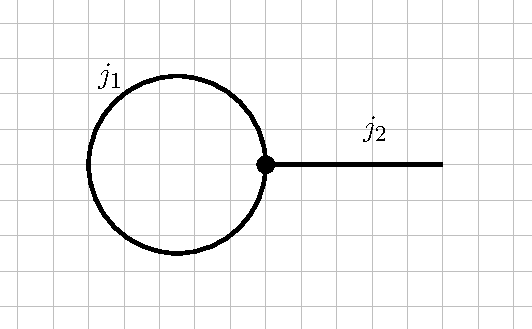
\includegraphics[width=69mm]{Graphs/1loop.pdf}
    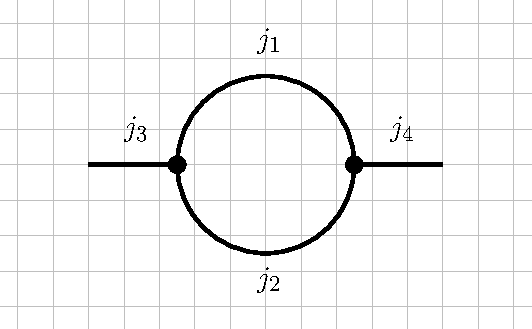
\includegraphics[width=69mm]{Graphs/2loop.pdf}
    \caption{Pictorial representation of the summation over projections. 3-$j$-symbols correspond to vertices, while angular momentum vectors are represented by edges. Left diagram corresponds to~\eqref{1loop}, where collapsing a 1-loop gives a factor of $\sqrt{(2j+1)}$, while the right diagram corresponds to~\eqref{2loop}, where collapsing a 2-loop produces a Kronecker delta function.}
    \label{fig:loops}
\end{figure}

\section{3j-symbols}
\label{app:3j}

Wigner 3-$j$ symbols are the coefficients with which three angular momenta must be added so that the resultant is zero. Most importantly for our purposes, they appear in the integral of three spherical harmonics~\eqref{3jInt}. For angular momentum vectors $j_1,j_2,j_3$ and their projections $m_1,m_2,m_3$, the 3-$j$ symbols are usually written in the form
\begin{equation}
    \begin{pmatrix} j_1 & j_2 & j_3 \\ m_1 & m_2 & m_3 \end{pmatrix}
\end{equation}
The closed-form expression evaluating a general 3-$j$ symbol is rather involved, but tabulate values can be found for example in~\cite{}. The necessary condition for a non-zero value are as follows:
\begin{itemize}
    \item $m_1+m_2+m_3 =0$,
    \item $j_1,j_2,j_3$ satisfy the triangle condition,
    \item $j_1+j_2+j_3$ is an integer (even integer if $m_1=m_2=m_3=0$).
\end{itemize}
Furthermore, permutation of any of the columns gives a factor of $(-1)^{j_1+j_2+j_3}$.

Summation over the projections in a product of 3-$j$ symbols can be conveniently represented graphically, with momenta $j$ represented by edges and 3-$j$ symbols by nodes. A shared edge denotes a shared value of $j$ with an opposite value of $m$. The summing over all $m$ then corresponds to collapsing subsequent loops in the resulting diagram. Each 1-loop gives a factor of $\sqrt{2j+1}$ and forces the remaining edge to be zero, while each 2-loop gives a Kronecker delta of the two outgoing edges. In the following we present the first few distinct cases. The sum over $m$ denotes summation over all $m_i$ indices..

Summing a single 3-$j$ symbol connected to itself, means collapsing a single 1-loop. The result is
\begin{equation}\label{1loop}
    \sum_m (-1)^{j_1-m_1}\begin{pmatrix} j_1 & j_1 & j_2 \\ -m_1 & m_1 & m_2\end{pmatrix} = \delta_{j_2,0}\sqrt{2j_1+1}.
\end{equation}
Summing over a pair of 3-$j$ symbols results in a product of two 1-loops or a single 2-loop:
\begin{align}
    &\sum_{m}(-1)^{m_1+m_2+m_3}
    \begin{pmatrix} j_1 & j_1 & j_3 \\ -m_1 & m_1 & -m_3 \end{pmatrix}
    \begin{pmatrix} j_2 & j_2 & j_4 \\ -m_2 & m_2 & m_4 \end{pmatrix} \nonumber
    \\
   & \mspace{250mu} = \delta_{j_3,0}\delta_{j_4,0}\sqrt{(2j_1+1)(2j_2+1)},\\
    &\sum_{m}(-1)^{m_1+m_2+m_3}
    \begin{pmatrix} j_1 & j_2 & j_3 \\ -m_1 & -m_2 & -m_3 \end{pmatrix}
    \begin{pmatrix} j_1 & j_2 & j_4 \\ m_1 & m_2 & m_4 \end{pmatrix}
    = \delta_{j_3,j_4}.\label{2loop}
\end{align}
The two situations~\eqref{1loop} and~\eqref{2loop} are presented in figure~\ref{fig:loops}. 

\begin{figure}
    \centering
    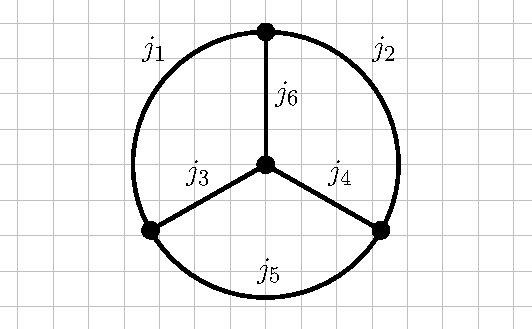
\includegraphics[width=69mm]{Graphs/6j.pdf}
    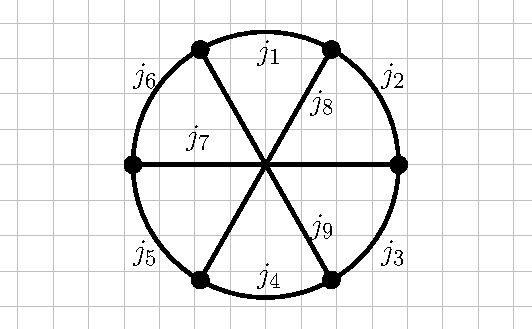
\includegraphics[width=69mm]{Graphs/9j.pdf}
    \caption{Pictorial representation of~\eqref{6j} resulting in a $6j-$symbol (left) and of~\eqref{9j}  resulting in a 9-$j$ symbol (right). In the right diagram there is no vertex in the middle\footnotemark. Notice that no 1-loops or 2-loops are present and so both of these do not simplify to combinations of Kronecker delta functions.}
    \label{fig:jsymbols}
\end{figure}
\footnotetext{There is no planar representation of such a graph, as it is isomorphic to the utility graph $K_{3,3}$~\cite{trudeau1993introduction}.}

Summation of three 3-$j$ symbols can always be performed by collapsing 1- and 2-loops, since the total number of legs is odd. The first non-trivial case happens with four interconnected 3-$j$ symbols in the form
\begin{align}\label{6j}
   \sum_m(-1)^\xi&\left(\begin{matrix}j_1&j_2&j_3\\-m_1&-m_2&-m_3\end{matrix}\right)\left(\begin{matrix}j_1&j_5&j_6\\m_1&-m_5&m_6\end{matrix}\right) \nonumber\\
   &\times\left(\begin{matrix}j_4&j_2&j_6\\m_4&m_2&-m_6\end{matrix}\right)\left(\begin{matrix}j_4&j_5&j_3\\-m_4&m_5&m_3\end{matrix}\right) =  \bigg\{\begin{matrix}j_1&j_2&j_3\\j_4&j_5&j_6\end{matrix}\bigg\}.
\end{align}
where $\xi = \sum_i (j_i-m_i)$. This quantity is called a 6-$j$ symbol for the purpose of tabulating values, as it does not reduce to a simple expression~\cite{biedenharn1984angular}. Similarly a product of 6 3-$j$ symbols can produce a 9-$j$ symbol
\begin{align}\label{9j}
   \sum_m(-1)^\xi&\left(\begin{matrix}j_1&j_2&j_3\\-m_1&-m_2&-m_3\end{matrix}\right)\left(\begin{matrix}j_4&j_5&j_6\\-m_4&-m_5&-m_6\end{matrix}\right) \nonumber\\
   &\mspace{50mu}\times\left(\begin{matrix}j_7&j_8&j_9\\-m_7&-m_8&-m_9\end{matrix}\right)\left(\begin{matrix}j_1&j_4&j_7\\m_1&m_4&m_7\end{matrix}\right) \nonumber
   \\
   &\mspace{50mu}\times\left(\begin{matrix}j_2&j_5&j_8\\m_2&m_5&m_8\end{matrix}\right)\left(\begin{matrix}j_3&j_6&j_9\\m_3&m_6&m_9\end{matrix}\right) =  \left\{\begin{matrix}j_1&j_2&j_3\\j_4&j_5&j_6\\j_7&j_8&j_9\end{matrix}\right\}.
\end{align}
Both of these are illustrated in figure~\ref{fig:jsymbols}. The exist  for evaluating the $6j-$ and 9-$j$ symbols can be performed with recursive algorithms analogous to the one used for 3-$j$ symbols~\cite{jsymbolsRef}.

